\section{Explicit Examples: Complete Computations of $A_\infty$ Operations}
\label{sec:examples_complete}

Three examples give the full $\Ainf$ operation tower $\{m_k\}_{k \ge 1}$ with integral evaluations and Stasheff identity verification.
\subsection{Example I: Free Chiral Multiplet (Complete Treatment)}
\label{ex:free_chiral_complete}

\subsubsection{Field Content and Classical Action}
A free chiral multiplet on $\R_t \times \C_z$ consists of a complex scalar field $\phi$ (in cohomological degree~$0$) and its BV antifield $\psi$ (in cohomological degree~$1$). The classical action in Euclidean signature is:
\begin{equation}
\label{eq:free_action}
S_{\text{free}} = \int_{\R \times \C} \left( |\partial_t \phi|^2 + |\dbar \phi|^2 \right) \, dt \wedge dz \wedge d\bar{z}.
\end{equation}
After holomorphic-topological twist, the BV action becomes:
\begin{equation}
S_{\text{HT}} = \int_{\R \times \C} \psi \,(\dbar + d_t)\, \phi \, dt \wedge dz \wedge d\bar{z}.
\end{equation}
\subsubsection{BV-BRST Complex}

In the BV formalism, the field $\phi$ (degree~$0$) is paired with the antifield $\psi$ (degree~$1$) via the BV bracket:
\begin{equation}
\{\phi(x), \psi(y)\}_{\mathrm{BV}} = \delta^{(3)}(x-y).
\end{equation}
The BV-BRST differential $Q = \{S_{\text{HT}}, \cdot\}_{\mathrm{BV}}$ acts on local observables $\A_{\text{free}} = \C[\phi_n, \psi_n \mid n \geq 0]$ by
\begin{align}
Q \cdot \phi_n &= \psi_n, \label{eq:Q_free_phi} \\
Q \cdot \psi_n &= 0, \label{eq:Q_free_psi}
\end{align}
with $Q^2\phi_n = Q(\psi_n) = 0$.

Here $\phi_n = \frac{1}{n!} \partial_z^n \phi$ is the $n$th holomorphic derivative.
\subsubsection{Propagator and Two-Point Function}
The free propagator in HT gauge is the Green's function for the kinetic operator $d_t + \dbar$:
\begin{equation}
\label{eq:free_propagator}
\langle \phi(t_1, z_1) \psi(t_2, z_2) \rangle = \frac{1}{2\pi} \cdot \frac{\Theta(t_1 - t_2)}{z_1 - z_2}.
\end{equation}
In the holomorphic direction
\begin{equation}
\label{eq:free_propagator_holo}
\langle \phi(z_1) \psi(z_2) \rangle_{\text{holo}} = \frac{1}{z_1 - z_2}.
\end{equation}

\subsubsection{Computing $m_2$: The $\lambda$-Bracket}
The binary operation $m_2$ comes from the two-point function. For observables $O_1 = \phi$ and $O_2 = \psi$:
\begin{equation}
m_2(\phi(z_1), \psi(z_2)) = \oint_{|z_1 - z_2| = \varepsilon} \langle \phi(z_1) \psi(z_2) \rangle \, \frac{dz_1}{z_1 - z_2}.
\end{equation}

By the propagator \eqref{eq:free_propagator_holo}
\begin{equation}
m_2(\phi, \psi) = \frac{1}{(z_1 - z_2)},
\end{equation}
so the $\lambda$-bracket is
\begin{equation}
\label{eq:free_lambda_bracket}
\{\phi_\lambda \psi\} = 1.
\end{equation}

On cohomology, since $(\phi_n, \psi_n)$ are acyclic doublets with $H^\bullet = \C$, the descended $\lambda$-bracket is trivial:
\begin{equation}
\{\cdot_\lambda \cdot\}_{\text{coh}} = 0.
\end{equation}

\subsubsection{Free-Theory Truncation}

\begin{proposition}[All $m_{k \geq 3} = 0$ for Free Theory]
\label{prop:free_higher_vanish}
In the free chiral multiplet theory, all higher operations $m_k = 0$ for $k \geq 3$.
\end{proposition}

\begin{proof}
Higher operations $m_k$ arise from Feynman diagrams with $k$ external legs. For $k \geq 3$, such diagrams require at least one internal vertex; the free theory has \textbf{no interaction vertices} (the action is quadratic). Diagrams contributing to $m_{k \geq 3}$ vanish identically.

Algebraically, the free propagator $\langle \phi(z_1)\psi(z_2)\rangle$ satisfies
\begin{equation}
Q \cdot \text{Prop}(z_1, z_2) = 0 \quad \text{(on-shell)},
\end{equation}
and no cubic or higher vertices generate internal structure.
\end{proof}

\subsubsection{Cohomology and PVA Structure}

\begin{proposition}[Cohomology of Free Theory]
\label{prop:free_cohomology_complete}
The cohomology $H^\bullet(\A_{\text{free}}, Q)$ is:
\begin{equation}
H^\bullet(\A_{\text{free}}, Q) = \C,
\end{equation}
concentrated in degree~$0$ and generated by the constant~$1$.
\end{proposition}

\begin{proof}
By \eqref{eq:Q_free_phi}--\eqref{eq:Q_free_psi},
\begin{equation}
Q \cdot \phi_n = \psi_n, \quad Q \cdot \psi_n = 0,
\end{equation}
giving the two-term chain complex
\begin{equation}
\A_{\text{free}} : \quad \C[\phi_n] \xrightarrow{Q} \C[\psi_n] \xrightarrow{Q} 0.
\end{equation}

Each pair $(\phi_n, \psi_n)$ is an acyclic doublet ($Q$ maps $\phi_n$ isomorphically to $\psi_n$), so
\begin{equation}
H^0 = \C, \quad H^{k} = 0 \text{ for } k \neq 0.
\end{equation}
\end{proof}
Since $m_{k \geq 3} = 0$ (Proposition \ref{prop:free_higher_vanish}), the structure on $H^\bullet(\A_{\text{free}}, Q)$ is a \emph{commutative vertex algebra} (a PVA with trivial bracket).

\subsubsection{Sesquilinearity Verification}

The sesquilinearity axioms \eqref{eq:sesqui_explicit_1}--\eqref{eq:sesqui_explicit_k} for the free theory.
\begin{lemma}[Sesquilinearity for Free Theory]
\label{lem:free_sesquilinearity}
The $\lambda$-bracket $\{\phi_\lambda \psi\} = 1$ satisfies sesquilinearity:
\begin{align}
\{\partial \phi_\lambda \psi\} &= -\lambda \{\phi_\lambda \psi\} = -\lambda, \\
\{\phi_\lambda \partial \psi\} &= (\partial + \lambda) \{\phi_\lambda \psi\} = \lambda.
\end{align}
\end{lemma}

\begin{proof}
Sesquilinearity follows from the translation equivariance of the propagator:
\begin{equation}
\partial_{z_1} \left( \frac{1}{z_1 - z_2} \right) = -\frac{1}{(z_1 - z_2)^2},
\end{equation}
which encodes the $-\lambda$ factor in the first identity. The second identity follows from differentiation in $z_2$.
\end{proof}

\subsection{Example II: Landau--Ginzburg Cubic Superpotential}
\label{lem:LG_cubic_complete}

The Landau--Ginzburg (LG) model with cubic superpotential $W(\phi) = \frac{1}{3} \phi^3$ is the first example with nontrivial higher operations.

\subsubsection{Action and Interaction Vertex}

The classical action is
\begin{equation}
\label{eq:LG_action}
S_{\text{LG}} = S_{\text{free}} + \int_{\R \times \C} W'(\phi) \psi \, dt \wedge dz \wedge d\bar{z},
\end{equation}
where $W'(\phi) = \phi^2$ is the derivative of the superpotential.

The interaction term produces a \textbf{cubic vertex}
\begin{equation}
\text{Vertex} = \int \phi^2 \psi \, dt \, dz \, d\bar{z}.
\end{equation}

\subsubsection{BV-BRST Differential}

On the algebra of local observables $\A_{\text{LG}} = \C[\phi_n, \psi_n]$, the BV-BRST differential decomposes into a linear part (identical to the free theory) and an interaction part from the superpotential:
\begin{align}
m_1(\phi_n) &= \psi_n + W'(\phi_n) = \psi_n + \lambda_3 \phi_n^2, \label{eq:Q_LG_phi} \\
m_1(\psi_n) &= 0. \label{eq:Q_LG_psi}
\end{align}
Nilpotency $m_1^2 = 0$ follows from the BV master equation $\{S_{\mathrm{BV}}, S_{\mathrm{BV}}\} = 0$ on the full BV complex including antifield pairings. The linear part $Q(\phi_n) = \psi_n$ is the differential of the free theory; the superpotential contributes $W'(\phi) = \lambda_3\phi^2$ to $m_1$, so the cohomology is the Jacobian ring $J(W) = \C[\phi]/(\lambda_3 \phi^2)$ rather than the free-theory cohomology~$\C$.

\subsubsection{Computing $m_2$: Modified $\lambda$-Bracket}

The binary operation $m_2$ receives corrections from the superpotential. The two-point function is
\begin{equation}
m_2(\phi, \phi) = \frac{1}{z_1 - z_2} + \text{(quantum corrections)}.
\end{equation}

At tree level (classical), the $\lambda$-bracket is
\begin{equation}
\{\phi_\lambda \phi\}_{\text{tree}} = \frac{\partial W'}{\partial \phi} = \phi^2.
\end{equation}

\subsubsection{Computing $m_3$: The Higher Operation}

The operation $m_3$ arises from the tree-level Feynman diagram with three external legs and one internal cubic vertex (a \textbf{Y-graph}):

\begin{center}
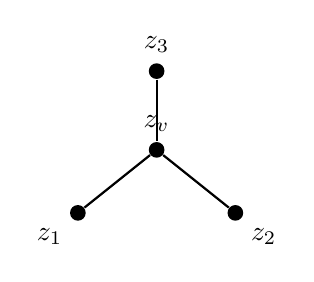
\begin{tikzpicture}
\node[circle, fill, inner sep=2pt, label=above:{$z_v$}] (v) at (1,0.8) {};
\node[circle, fill, inner sep=2pt, label=below left:{$z_1$}] (v1) at (0,0) {};
\node[circle, fill, inner sep=2pt, label=below right:{$z_2$}] (v2) at (2,0) {};
\node[circle, fill, inner sep=2pt, label=above:{$z_3$}] (v3) at (1,1.8) {};

\draw[thick] (v1) -- (v);
\draw[thick] (v2) -- (v);
\draw[thick] (v3) -- (v);
\end{tikzpicture}
\end{center}

Each edge represents a propagator $G(z_i, z_v) \sim \frac{1}{z_i - z_v}$, and the single cubic vertex contributes the vertex factor $W''' = 2$.

\begin{proposition}[Explicit Formula for $m_3$]
\label{prop:LG_m3_formula}
Let\/ $\cA$ be the LG cubic model with superpotential
$W(\phi) = \tfrac{1}{3}\phi^3$. Then
\begin{equation}
m_3(\phi, \phi, \phi) = W'''(0) = 2.
\end{equation}
\end{proposition}

\begin{proof}
The unique tree contributing to~$m_3$ is the Y-graph
(Theorem~\ref{thm:physics-bridge}, Lemma~\ref{lem:QME_to_Ainfty}).
On cohomology $H^\bullet(\cA, Q) = \C$, the homotopy transfer formula gives
\[
 m_3^H = p \circ m_3 \circ \iota^{\otimes 3}
 - p \circ m_2 \circ (h \circ m_2 \otimes \iota
 + \iota \otimes h \circ m_2) \circ \iota^{\otimes 3}.
\]
For constant-mode inputs, $m_2(\iota(1), \iota(1)) \in \ker h$ (the product of constants is constant), so the correction terms vanish and $m_3^H = W'''(0) = 2$.
\end{proof}

\subsubsection{FM boundary structure and the Arnold relation}

\begin{computation}[Y-graph boundary analysis]
\label{comp:m3_residue}
Consistency of $m_3 = 2$ with the FM boundary structure.

\textbf{FM compactification of the Y-graph.}
The Y-graph diagram lives on $\FM_4(\C)$ (three external points $z_1, z_2, z_3$ plus the internal vertex $z_v$). The relevant boundary divisors are $D_{\{i,v\}}$ for $i = 1, 2, 3$, where $z_v$ collides with an external point.

\textbf{Residue at \(D_{\{1,v\}}\).}
Near $D_{\{1,v\}}$, set $z_v = z_1 + \varepsilon$, $\varepsilon \to 0$. The Y-graph integrand becomes
\begin{equation}
\frac{1}{\varepsilon \cdot (z_2 - z_1 - \varepsilon)
 (z_3 - z_1 - \varepsilon)}
\;\xrightarrow{\;\varepsilon \to 0\;}
\;\frac{1}{\varepsilon \cdot (z_2 - z_1)(z_3 - z_1)}.
\end{equation}
The residue at $\varepsilon = 0$ is $1/[(z_2 - z_1)(z_3 - z_1)]$, contributing the binary composition $m_2(m_2(\phi_1, \phi_v), \phi_2, \phi_3)$ in the Stasheff relation. Summing all three boundary strata:
\begin{equation}
W''' \sum_{\text{cyc}} \Res_{D_{\{i,v\}}}
= 2 \left[
 \frac{1}{(z_2 - z_1)(z_3 - z_1)}
 + \frac{1}{(z_1 - z_2)(z_3 - z_2)}
 + \frac{1}{(z_1 - z_3)(z_2 - z_3)}
\right] = 0.
\end{equation}

\textbf{Arnold relation.}
The vanishing of the boundary sum is the partial-fraction identity $\sum_{\text{cyc}} 1/[(z_j - z_i)(z_k - z_i)] = 0$, an instance of the Arnold relation on $\FM_4(\C)$ (Theorem~\ref{thm:Arnold_full_proof}). The Arnold relation constrains the \emph{compositions} $m_2 \circ m_2$ that appear in the Stasheff identity $\sum m_i \circ m_j = 0$, not the value of~$m_3$ itself. The operation $m_3 = W''' = 2$ is extracted from the vertex factor (Proposition~\ref{prop:LG_m3_formula}); the Arnold relation ensures the degree-$3$ Stasheff identity $m_1 \circ m_3 + m_2 \circ m_2 + m_3 \circ m_1 = 0$.
\end{computation}

\subsubsection{Cubic minimal-model truncation}

\begin{theorem}[Cubic Landau--Ginzburg minimal-model truncation]
\label{thm:LG_truncation}
Let\/ $\cA$ be a logarithmic\/ $\SCchtop$-algebra.
For the one-variable Landau--Ginzburg model with cubic superpotential
$W(\phi)=\phi^3/3$, the minimal transferred \(A_\infty\)-structure on
the Jacobi ring \(J(W)=\C[\phi]/(\phi^2)\) satisfies
\begin{equation}
m_k=0\qquad(k\geq 4),
\end{equation}
and its only non-binary higher operation is
\(m_3(\phi,\phi,\phi)=W'''=2\).
\end{theorem}

\begin{proof}
Let \(\pi:\C[\phi]\to J(W)\) be the Jacobi projection and let \(h\)
be the contracting homotopy on the ideal \((\phi^2)\). The
homological perturbation formula writes \(m_n^J\) as a sum over rooted
trees whose vertices are the Taylor tensors \(W^{(r)}\), whose internal
edges are \(h\), and whose root is followed by \(\pi\). Since
\[
W'''=2,\qquad W^{(r)}=0\quad(r\geq4),
\]
the only one-vertex tree beyond multiplication is the cubic corolla,
and it gives \(m_3^J(\phi,\phi,\phi)=2\). Every tree with at least two
cubic vertices has an internal cubic edge. Its root contribution lies
in \((\phi^2)\), hence is annihilated by \(\pi\). Thus no rooted tree
with \(n\geq4\) survives in the minimal model.
\end{proof}

\begin{remark}[Higher Taylor tensors]
For superpotentials with higher-degree terms (e.g., $W(\phi) = \frac{1}{3}\phi^3 + \frac{1}{5}\phi^5$), $W''' \neq \text{const}$ and $W^{(5)} \neq 0$ enable higher operations $m_k$ at larger $k$. The truncation at $k=4$ is specific to the \textbf{cubic} case.
\end{remark}

\subsubsection{Cohomology and PVA Structure}

\begin{proposition}[Cohomology of LG Cubic]
The full $A_\infty$ differential $m_1$ acts by multiplication by $W'(\phi) = \lambda_3 \phi^2$, so
the cohomology is the Jacobian ring
\begin{equation}
H^\bullet(\A_{\text{LG}}, m_1) \;\cong\; J(W) = \C[\phi]/(W'(\phi)) = \C[\phi]/(\lambda_3 \phi^2),
\end{equation}
a $2$-dimensional algebra with basis $\{1, \phi\}$.
(The higher modes $(\phi_n, \psi_n)$ for $n \geq 2$ form acyclic $m_1$-doublets.)
The homotopy-transferred $A_\infty$ structure on $J(W)$ inherits a nonvanishing ternary
operation $m_3^{J(W)}$ encoding the residual cubic coupling.
\end{proposition}

\subsection{Example III: Abelian Gauge Theory with Chern--Simons}
\label{prop:abelian_CS_complete}

The third example is abelian $U(1)$ gauge theory with Chern--Simons coupling at level $k \in \Z$.

\subsubsection{Action and Field Content}

The fields are:
\begin{itemize}
\item Gauge field $A \in \Omega^1(\R \times \C)$,
\item Ghost $c$ and antighost $\bar{c}$ (from gauge fixing).
\end{itemize}

The action is:
\begin{equation}
\label{eq:CS_action}
S_{\text{CS}} = \frac{k}{4\pi} \int_{\R \times \C} A \wedge dA + \text{(gauge fixing terms)}.
\end{equation}

In HT gauge, this becomes:
\begin{equation}
S_{\text{HT-CS}} = \frac{k}{2\pi} \int A_z \, d_t A_{\bar{z}} + \bar{c} \, d_t c.
\end{equation}

\subsubsection{Bulk Local Operators}

The bulk local operators are generated by:
\begin{equation}
\A_{\text{bulk}} = \C[J_n \mid n \in \Z],
\end{equation}
where $J_n = \frac{1}{n!} \partial_z^n A_z$ are holomorphic derivatives of the gauge field component $A_z$.

\subsubsection{BV-BRST Differential}

The BV-BRST differential acts by:
\begin{equation}
Q \cdot A = d_t c, \quad Q \cdot c = 0.
\end{equation}

This defines a chain complex with cohomology:
\begin{equation}
H^\bullet(\A_{\text{bulk}}, Q) = \C[J_n \mid n \in \Z].
\end{equation}

\subsubsection{$\lambda$-Bracket and Affine Kac--Moody Structure}

The $\lambda$-bracket on $H^\bullet(\A_{\text{bulk}}, Q)$ is computed from the CS propagator:
\begin{equation}
\langle A_z(z_1) A_{\bar{z}}(z_2) \rangle = \frac{k}{2\pi} \cdot \frac{1}{z_1 - z_2}.
\end{equation}

This yields the PVA $\lambda$-bracket:
\begin{equation}
\{J_\lambda J\} = k\lambda,
\end{equation}
encoding the double-pole OPE $J(z)J(w) \sim k/(z-w)^2$.
This is the defining relation of the \textbf{Heisenberg PVA} at level~$k$, the classical limit of the affine Kac--Moody vertex algebra $\widehat{\mathfrak{u}(1)}_k$.

\subsubsection{Boundary Conditions and WZW Model}

Impose boundary conditions on $\R \times \C$ along the half-space $\{t \geq 0\} \times \C$.

\textbf{Neumann boundary}: $\left. \frac{\partial A}{\partial t} \right|_{t=0} = 0$ produces a boundary \textbf{vertex algebra}
\begin{equation}
\mathcal{V}_{\text{Neumann}} = \text{(Heisenberg vertex algebra at level $k$)}.
\end{equation}

\textbf{Dirichlet boundary}: $A|_{t=0} = \text{const}$ produces
\begin{equation}
\mathcal{V}_{\text{Dirichlet}} = \text{(WZW model for $U(1)$ at level $k$)}.
\end{equation}

These boundary chiral algebras are analyzed in \cite{CDG20}.

\subsubsection{Higher Operations and Quantum Corrections}

\begin{proposition}[No Quantum Corrections in Abelian CS]
Let\/ $\cA$ be a logarithmic\/ $\SCchtop$-algebra.
For abelian $U(1)$ Chern--Simons theory, all higher operations $m_{k \geq 3} = 0$ at the quantum level.
\end{proposition}

\begin{proof}
Abelian CS is a \textbf{free theory} (no interaction vertices in the action). Feynman diagrams beyond tree level require internal vertices; abelian gauge fields have none. Thus
\begin{equation}
m_k = 0 \quad \text{for all } k \geq 3.
\end{equation}
For non-abelian gauge theories, self-interactions of gauge fields generate higher $m_k$.
\end{proof}

\subsubsection{Connection to Quantum Groups}

For non-abelian groups $G$, the same construction gives
\begin{equation}
\mathcal{A}_{\partial} = \text{(affine Kac--Moody PVA for $\mathfrak{g}$ at level $k$)},
\end{equation}
as the boundary current chart.  Under the physics bridge and the
boundary-linear exact-sector comparison, the associated bulk object is
the chiral derived centre
$C^\bullet_{\mathrm{ch}}(\mathcal{A}_{\partial},\mathcal{A}_{\partial})$.
Line operators generate \textbf{Yangian algebras}
(Section \ref{sec:line_operators}).

\subsection{Summary Table of Examples (Proved)}

\begin{center}
\begin{tabular}{|l|c|c|c|c|}
\hline
\textbf{Theory} & $m_2$ & $m_3$ & $m_{k \geq 4}$ & $H^\bullet(\A, Q)$ \\
\hline
Free chiral & $\frac{1}{z_{12}}$ & $0$ & $0$ & $\C$ (trivial) \\
\hline
LG cubic & $\frac{1}{z_{12}} + O(\phi^2)$ & $\neq 0$ (truncates) & $0$ & $J(W) = \C[\phi]/(\phi^2) \cong \C^2$ \\
\hline
Abelian CS & $\frac{k}{z_{12}}$ & $0$ & $0$ & $\widehat{\mathfrak{u}(1)}_k$ \\
\hline
\end{tabular}
\end{center}

%%%%%%%%%%%%%%%%%%%%%%%%%%%%%%%%%%%%%%%%%%%%%%%%%%%%%%%%%%%%%%%%%%%%%%%%%%%%%
\subsection{SQCD: the first nonabelian gauge theory test}
\label{subsec:sqcd-nonabelian-test}
\index{SQCD|textbf}
\index{boundary algebra!nonabelian gauge theory}
%%%%%%%%%%%%%%%%%%%%%%%%%%%%%%%%%%%%%%%%%%%%%%%%%%%%%%%%%%%%%%%%%%%%%%%%%%%%%

\providecommand{\QBRST}{Q_{\mathrm{BRST}}}

$\mathrm{SU}(N)$ SQCD with $N_f$ fundamental chirals is the first nonabelian gauge theory example, following Costello--Dimofte--Gaiotto
\cite{CDG2023}, \S6.5.

\paragraph{Field content and boundary conditions.}
The bulk theory is $3$d $\cN=4$ $\mathrm{SU}(N)$ gauge theory coupled to $N_f$ chiral multiplets $(X^i, \Psi_i)$ ($i = 1, \ldots, N_f$) in the fundamental representation, with Neumann boundary conditions for the gauge field. After the HT twist the boundary supports
\begin{itemize}
\item a gauged $\beta\gamma$ system in the adjoint representation (ghosts $b, c$);
\item matter fields $(X^i, \Psi_i)$ in the fundamental of $\mathrm{SU}(N)$, forming a $\beta\gamma$ system for each flavor.
\end{itemize}

\paragraph{BRST charge.}
The boundary BV-BRST differential is
\begin{equation}\label{eq:sqcd-brst}
 \QBRST \;=\; \oint\!\Bigl(
 \operatorname{Tr}\bigl(c \cdot [\text{adj.\ fields}]\bigr)
 + \tfrac{1}{2}\operatorname{Tr}(b\, c^2)
 + \Psi_i\, c \cdot X^i
 \Bigr),
\end{equation}
where the first term implements the gauge constraint on adjoint fields,
the second is the standard ghost self-coupling ensuring $\QBRST^2 = 0$,
and the third couples the gauge ghosts to the matter sector.

\paragraph{Boundary algebra as bar cohomology.}
\begin{proposition}[SQCD boundary algebra]
\label{prop:sqcd-boundary-algebra}
\textup{(Costello--Dimofte--Gaiotto \cite{CDG2023}, \S6.5.)}
The boundary vertex algebra of $\mathrm{SU}(N)$ SQCD is the BRST
cohomology
\[
 \cA_\partial^{\mathrm{SQCD}}
 \;=\;
 H^\bullet\!\bigl(
 \beta\gamma^{\mathrm{adj}} \otimes (bc)^{\mathrm{adj}}
 \otimes \beta\gamma^{\mathrm{fund},\, \otimes N_f},\;
 \QBRST
 \bigr).
\]
The BRST differential $\QBRST$ coincides with the bar differential of
the gauge chiral algebra: gauge-invariant operators are precisely the
bar cohomology $H^\bullet(\bar{B}(\cA_{\mathrm{gauge}}))$.
\end{proposition}

\paragraph{Large-$N_f$ limit.}
For $N_f \gg N$, massive modes decouple and the BRST cohomology simplifies: the adjoint ghosts become acyclic against the matter sector, leaving an effective description in terms of gauge-invariant composites (mesons $M^i{}_j = X^i \Psi_j$ and baryons).

\paragraph{The DetYZ model.}
Costello--Dimofte--Gaiotto \cite{CDG2023}, \S6.5 introduce an alternative boundary description, the DetYZ model, built from determinant operators. The equivalence between the BRST description and the DetYZ description is a quasi-isomorphism of vertex algebras, a check of bar-cobar inversion (Theorem~B of Volume~I, inversion on the Koszul locus) in the nonabelian gauge-theory setting.

\begin{remark}[Bar-cobar interpretation]
\label{rem:sqcd-bar-cobar}
The SQCD example illustrates the central thesis: the BRST differential
\emph{is} the bar differential, and gauge-invariant boundary operators
\emph{are} bar cohomology classes. The boundary algebra is $H^\bullet(\bar{B}(\cA))$, where $\cA$ is the pre-gauge chiral algebra. Bar-cobar inversion (Theorem~B) reconstructs the full chiral algebra from its gauge-invariant sector.
\end{remark}

\begin{example}[SQCD character formulas]
\label{ex:sqcd-characters}
\index{SQCD!character formulas}
\textup{(Costello--Dimofte--Gaiotto \cite{CDG2023}, \S6.5.)}
The boundary character of $\mathrm{SU}(N)$ SQCD with $N_f$
fundamental chirals takes the form
\begin{equation}\label{eq:sqcd-character}
 \chi_{\mathrm{SQCD}}^{N,N_f}(q)
 \;=\;
 \oint [da]_{N}\;
 \prod_{n \geq 1}
 \frac{\det_{\mathrm{adj}}(1 - q^n\,\mathrm{Ad}(a))^2}
 {\det_{\mathrm{fund}}(1-q^n\,a)^{N_f}
 \det_{\mathrm{fund}}(1-q^n\,a^{-1})^{N_f}},
\end{equation}
where $[da]_N$ is the Haar measure on the $\mathrm{SU}(N)$ maximal
torus. For $N_f \geq 2N$, the integral converges and the character
matches the Hilbert series of bar cohomology:
$\chi_{\mathrm{SQCD}}^{N,N_f}(q) = \sum_{n \geq 0} q^n\,\dim
H^n(\bar{B}(\cA_{\mathrm{SQCD}}))$.
\end{example}

\begin{remark}[$N_f$ dependence and Seiberg duality]
\label{rem:sqcd-seiberg-duality}
\index{Seiberg duality!SQCD}
The SQCD boundary algebra varies with $N_f$:
\begin{enumerate}[label=\textup{(\roman*)},nosep]
\item $N_f < N$: the theory confines and the boundary algebra is trivial (bar-acyclic);
\item $N_f = N$: the DetYZ model provides an equivalent description via determinant operators;
\item $N_f > 2N$: infrared-free regime; the boundary algebra stabilizes and the character formula \eqref{eq:sqcd-character} simplifies.
\end{enumerate}
At the level of bar complexes, Seiberg duality $\mathrm{SU}(N)_{N_f} \leftrightarrow \mathrm{SU}(N_f - N)_{N_f}$ is a quasi-isomorphism: $\bar{B}(\cA^{N,N_f}) \simeq \bar{B}(\cA^{N_f-N,N_f})$. In the Chriss--Ginzburg convolution framework of Volume~I, Seiberg duality is MC gauge equivalence in a strict dg~Lie chart \textup{(}with the invariant deformation object understood up to filtered $L_\infty$ quasi-isomorphism, Convention~\ref{conv:vol2-strict-models}\textup{)}: $\Theta_{\mathrm{SU}(N)} \sim_{\mathrm{MC}} \Theta_{\mathrm{SU}(N_f-N)}$ in the ambient algebra $\mathfrak{g}^{\mathrm{amb}}$. The shadow algebras are isomorphic, $\cA^{\mathrm{sh}}_{N,N_f} \cong \cA^{\mathrm{sh}}_{N_f-N,N_f}$, so modular invariants (modular characteristic~$\kappa$, discriminant~$\Delta$, contact classes) match across the duality.
\end{remark}

% NOTE: The full primitive packages for twisted holography, M2, and M5
% are developed in detail in the worked examples chapter
% (Sections~\ref{subsec:twisted-holography-primitive},
% \ref{subsec:twisted-M2-primitive}, and
% \ref{subsec:twisted-M5-primitive}).
% The following section (CS) complements those with the first
% nonabelian gauge theory example computed in full primitive-package form.

%%%%%%%%%%%%%%%%%%%%%%%%%%%%%%%%%%%%%%%%%%%%%%%%%%%%%%%%%%%%%%%%%%%%%%%%%%%%%
\subsection{Nonabelian Chern--Simons: the primitive package}
\label{subsec:cs-primitive-package}
\index{Chern--Simons!primitive package|textbf}
\index{affine Kac--Moody!primitive package}
\index{Wilson line!open category}
%%%%%%%%%%%%%%%%%%%%%%%%%%%%%%%%%%%%%%%%%%%%%%%%%%%%%%%%%%%%%%%%%%%%%%%%%%%%%

Let $G$ be a simple simply connected compact Lie group with Lie algebra $\fg = \operatorname{Lie}(G)$ and let $k$ be a positive integer (the level). Chern--Simons theory at level~$k$ on $\R_{\ge 0} \times \C$ with Nahm-pole boundary condition is a holomorphic-topological theory; the open/closed data is computed below. The six-fold primitive package $(\cC_{\mathrm{CS}}^{\mathrm{op}},\; b_{\mathrm{Dir}},\; A = V_k(\fg),\; Z,\; \Theta_{\mathrm{CS}},\; \operatorname{Tr})$ realises Theorem~\ref{thm:thqg-swiss-cheese} explicitly.

\subsubsection*{Boundary algebra}

The boundary algebra is the universal affine vertex algebra at
level~$k$:
\begin{equation}\label{eq:cs-boundary-algebra}
A \;=\; V_k(\fg).
\end{equation}
Generators: currents $\{J^a(z)\}_{a=1}^{\dim\fg}$ in conformal
weight~1.
The defining $\lambda$-bracket is
\begin{equation}\label{eq:cs-lambda-bracket}
\{J^a{}_\lambda J^b\}
\;=\;
f^{ab}{}_c\, J^c \;+\; k\,\delta^{ab}\,\lambda,
\end{equation}
where $f^{ab}{}_c$ are the structure constants of~$\fg$ in a basis
with $\operatorname{tr}(t^a t^b) = \delta^{ab}$ and $\delta^{ab}$
is the Killing form normalized so that the long root has
$|\alpha|^2 = 2$.
The OPE is
\[
J^a(z)\, J^b(w)
\;\sim\;
\frac{k\,\delta^{ab}}{(z-w)^2}
\;+\;
\frac{f^{ab}{}_c\, J^c(w)}{z-w}.
\]
The highest pole is quadratic:
the $\lambda$-bracket is at most linear in~$\lambda$.
By the PBW criterion (Volume~I, Proposition~\ref*{V1-prop:pbw-universality}),
$V_k(\fg)$ is chirally Koszul for all $k \ne -h^\vee$.

\subsubsection*{$\Ainf$ structure: finite Lie transfer}

The $\lambda$-bracket~\eqref{eq:cs-lambda-bracket} satisfies the Lie
conformal Jacobi identity. On the strict PBW surface the transferred
tower has no operations beyond the finite Lie stage:
\begin{equation}\label{eq:cs-mk-vanish}
m_k \;=\; 0
\qquad
\text{for all } k \ge 4.
\end{equation}
The support shadow depth is \(r^\Theta_{\max}=3\)
(class~$\mathbf{L}$, Lie/tree): the cubic support component is nonzero
(it detects the Lie bracket $f^{ab}{}_c$); the quartic contact invariant vanishes,
\begin{equation}\label{eq:cs-quartic-vanishes}
\mathfrak{Q}^{\mathrm{contact}}_{V_k(\fg)} \;=\; 0,
\end{equation}
since no Virasoro quartic wheel is present. The absence of a quartic
pole terminates the contact tower after the finite cubic Lie transfer.

\subsubsection*{Open category (primitive)}

\begin{definition}[CS Wilson-line category]
\label{def:cs-open-category}
\index{Wilson line!dg-category}
The open-sector factorization dg-category is
\begin{equation}\label{eq:cs-open-category}
\cC_{\mathrm{CS}}^{\mathrm{op}}
\;\simeq\;
V_k(\fg)\text{-}\mathbf{mod}^{\mathrm{dg}},
\end{equation}
the dg-category of modules over the affine vertex algebra
$V_k(\fg)$.
The vacuum boundary object is
$b_{\mathrm{Dir}} = V_k(\fg)$
(the vacuum module, viewed as an object of its own module
category).
\end{definition}

At generic $k$ (not admissible), the category is abelian and semisimple on the subcategory of integrable highest-weight modules $\{L(\lambda) : \lambda \in P_+^k\}$. At admissible levels, null vectors give the category a derived structure. The endomorphism algebra recovers the boundary: $\End(b_{\mathrm{Dir}}) = V_k(\fg)$.

\subsubsection*{Koszul dual and line operators}

The Koszul reflection is the chiral Chevalley--Eilenberg object of the
current algebra at the Feigin--Frenkel reflected level:
\begin{equation}\label{eq:cs-koszul-dual}
V_k(\fg)^!
\;\simeq\;
\operatorname{CE}^{\mathrm{ch}}\!\bigl(\widehat{\fg}_{k'}\bigr),
\qquad
k' = -k - 2h^\vee.
\end{equation}
The affine algebra $V_{k'}(\fg)$ is the current presentation of this
CE object; it is not the Koszul dual object itself.  Line operators
along $\R_{>0} \times \{0\}$ are modules over this reflected current
presentation
(Theorem~\ref{thm:lines_as_modules}).
The complementarity anti-symmetry holds:
$\kappaChHodge(V_k(\fg)) + \kappaChHodge(V_{k'}(\fg)) = 0$.

\subsubsection*{Bulk (derived center)}

The chiral derived center is the chiral Hochschild cochain
complex:
\begin{equation}\label{eq:cs-derived-center}
Z
\;=\;
\mathcal{Z}^{\mathrm{der}}_{\mathrm{ch}}(V_k(\fg))
\;:=\;
H^*\!\bigl(
 C^\bullet_{\mathrm{ch}}(V_k(\fg),\, V_k(\fg)),\;
 \delta
\bigr).
\end{equation}
By the Hochschild--Serre spectral sequence for the
$\fg$-action:
\begin{equation}\label{eq:cs-hochschild-computation}
\mathcal{Z}^0
\;\simeq\;
Z(\widehat{\fg}_k)
\;=\;
\begin{cases}
\C & \text{if } k \ne -h^\vee, \\
\text{large} & \text{at critical level},
\end{cases}
\qquad
\mathcal{Z}^1
\;\simeq\;
H^1(\fg, V_k(\fg)),
\end{equation}
and, for a family datum $H_H(V_k(\fg);S_k)$, Theorem~H gives
$\mathcal Z^n\cong H^n(K_{V_k(\fg),S_k})$ with support in~$S_k$.
At generic non-critical level, $Z(\widehat{\fg}_k)=\C$ is the
degree-zero algebraic statement.  Under a perturbative
Chern--Simons/BV boundary comparison, its unit maps to the vacuum
summand of local closed observables.  Global flat-connection sectors,
framing dependence, and finite-level modular data belong to the
global three-dimensional input.  At the critical level
$k=-h^\vee$, the Feigin--Frenkel centre
$\mathfrak z(\widehat\fg)\cong
\operatorname{Fun}\operatorname{Op}_{\fg^L}(\mathbb D)$ enters the
degree-zero family model.

\subsubsection*{Classical $r$-matrix and coproduct}

The collision residue of the bar differential gives the
classical $r$-matrix (pole orders one below the OPE, since the $d\log$ bar kernel absorbs one pole):
\begin{equation}\label{eq:cs-r-matrix}
r^{\mathrm{coll}}_{\mathrm{CS}}(z)
\;=\;
\frac{k\,\Omega}{z},
\end{equation}
where $\Omega = \sum_a t^a \otimes t^a \in \fg \otimes \fg$ is the
quadratic Casimir and $k$ is the level.
The Laplace kernel (the full OPE generating function) is
$r^L(z) = f^{ab}{}_c J^c/z + k\,\delta^{ab}/z^2$.
The collision residue $k\,\Omega_{\mathrm{tr}}/z$ satisfies the CYBE:
\begin{equation}\label{eq:cs-cybe}
[k\,\Omega_{12}/z_{12},\; k\,\Omega_{13}/z_{13}]
+ [k\,\Omega_{12}/z_{12},\; k\,\Omega_{23}/z_{23}]
+ [k\,\Omega_{13}/z_{13},\; k\,\Omega_{23}/z_{23}]
\;=\; 0.
\end{equation}
This is the standard rational CYBE (the common factor $k^2$ cancels); the solution $k\,\Omega_{\mathrm{tr}}/z$
is the classical rational residue underlying the affine
KZ/Drinfeld--Kohno comparison surface.

The coproduct on the dg-shifted Yangian is nontrivial:
\begin{equation}\label{eq:cs-coproduct}
\Delta_z(J^a)
\;=\;
J^a(w+z) \otimes 1
\;+\;
1 \otimes J^a(w),
\end{equation}
and on composite operators the coproduct is a strict algebra morphism into the $r(z)$-twisted tensor product. $\Delta_z$ is non-primitive on composites: the $r(z)$-twist encodes the braiding of Wilson lines. CS gluons \emph{split}: a Wilson line in representation~$R$ passing through two regions separated by a bulk excitation resolves into constituent Wilson lines weighted by the tensor product decomposition $R \to \bigoplus R_i \otimes R_j$, the Clebsch--Gordan coupling.

In contrast, gravity (\S\ref{subsec:gravity-primitive-package}) has a ghost-number obstruction that forces the Virasoro coproduct to be strictly primitive; the obstruction is absent here because the affine generators $J^a$ are weight~1 (matching the SDR image), while the Sugawara composite $T$ is weight~2 (outside the SDR image).

\subsubsection*{Modular MC element}

\begin{theorem}[CS modular MC element]
\label{thm:cs-mc-element}
\index{universal MC element!Chern--Simons|textbf}
The modular MC element of $V_k(\fg)$ is
\begin{equation}\label{eq:cs-mc-element}
\Theta_{\mathrm{CS}}
\;=\;
\alpha_{\mathrm{cl}}
\;+\;
\hbar\,\kappa\,\eta \otimes \Lambda,
\end{equation}
where:
\begin{enumerate}[label=\textup{(\roman*)}]
\item $\alpha_{\mathrm{cl}} = m_2 \in
 \Hom(\barB^{(0,2)}(\SCop), \End_{V_k(\fg)})$
 encodes the binary $\lambda$-bracket at genus~$0$.
 The MC equation at genus~$0$ is
 $d_{\barB}\alpha_{\mathrm{cl}}
 + \frac{1}{2}[\alpha_{\mathrm{cl}}, \alpha_{\mathrm{cl}}] = 0$,
 which is the Jacobi identity for the Lie bracket.
\item $\hbar\,\kappa\,\eta \otimes \Lambda$ is the genus-$1$
 self-loop correction, with modular characteristic
 \begin{equation}\label{eq:cs-kappa}
 \kappaChHodge(V_k(\fg))
 \;=\;
 \frac{\dim(\fg)\cdot(k + h^\vee)}{2h^\vee}.
 \end{equation}
\item No primitive support coordinate occurs above the cubic
 Lie--Jacobi layer: $m_k = 0$ for $k \ge 4$
 forces all planted-forest corrections requiring an independent
 degree-$\ge4$ support vertex to vanish.  The scalar Hodge genus tower
 remains present.
\end{enumerate}
The bar-intrinsic support packet has support depth
\(r^\Theta_{\max}=3\) (class~$\mathbf{L}$):
\[
\Theta_{\mathrm{CS}}^{\le 2} = \kappa \cdot \eta \otimes \Lambda,
\qquad
\Theta_{\mathrm{CS}}^{\le 3} = \kappa \cdot \eta \otimes \Lambda
+ \mathfrak{C} \cdot \Xi_3,
\qquad
\Theta_{\mathrm{CS}}^{\le r} = \Theta_{\mathrm{CS}}^{\le 3}
\;\text{ for all } r \ge 3,
\]
where $\mathfrak{C}(\widehat{\fg}_k) \ne 0$ is the cubic shadow
(detecting the Lie bracket) and $\Xi_3$ is the degree-$3$
tautological form on $\overline{\mathcal{M}}_{0,3}$. This is a
support-packet statement, not an assertion that obstruction-class
vanishing determines the packet.
\end{theorem}

\begin{proof}
The binary operation $m_2$ satisfies the Lie conformal Jacobi identity,
so $\alpha_{\mathrm{cl}}$ satisfies the genus-$0$ MC equation. The
finite cubic transfer is the class $\mathfrak C$ above. The genus-$1$
scalar contribution is the self-loop graph $\Gamma_{\mathrm{irr}}$
\textup{(}one vertex, one self-edge\textup{)}, contributing
$\kappa \cdot \eta \otimes \Lambda$ with
$\kappa = \dim(\fg)(k + h^\vee)/(2h^\vee)$ from the BV trace
$\sum_a \langle J^a, J^a \rangle = k\dim(\fg)$ weighted by the Hodge
class $\omega_1 = \lambda_1/12$. Here
$\langle J^a, J^b \rangle = k\,\delta^{ab}$ is the level-$k$ pairing;
the $h^\vee$ correction comes from the shift between the Lie-algebra
trace and the vertex-algebra invariant bilinear form
(Volume~I, Proposition~\ref*{V1-prop:kappa-affine}).

Planted-forest corrections at degree $r \ge 4$ require an internal
vertex labelled by some $m_j$ with $j \ge 4$; since the class-$L$
transfer has no such vertex, these corrections vanish. At higher genus
$g \ge 2$, the same support cutoff applies: no primitive support
component of degree $\ge4$ occurs, while the scalar genus tower is
$F_g(V_k(\fg)) = \kappaChHodge(V_k(\fg))\lambda_g^{\mathrm{FP}}$, with
$\lambda_g^{\mathrm{FP}}=\int_{\overline{\mathcal{M}}_{g,1}}\psi_1^{2g-2}\lambda_g$,
by the algebraic-family rigidity theorem
(Volume~I, Theorem~\ref*{V1-thm:algebraic-family-rigidity}).
\end{proof}

\subsubsection*{Annulus trace}

The annulus trace is the chiral Hochschild homology of the open
chiral boundary sector:
\begin{equation}\label{eq:cs-annulus-trace}
\operatorname{Tr}_{\mathrm{CS}}
\;=\;
\int_{S^1} \cC_{\mathrm{CS}}^{\mathrm{op}}
\;\simeq\;
\HH^{\mathrm{ch}}_\bullet(V_k(\fg)).
\end{equation}
At rational $C_2$-cofinite levels, the Zhu comparison identifies
$\HH^{\mathrm{ch}}_0(V_k(\fg))$ with the trace of the identity on the
Zhu algebra quotient. For the universal affine algebra the Zhu algebra
is $A(V_k(\fg)) \simeq U(\fg)$; the character statement below uses the
integrable quotient.
The annulus partition function
\begin{equation}\label{eq:cs-annulus-partition}
Z_{\mathrm{ann}}^{\mathrm{CS}}(q)
\;=\;
\operatorname{tr}_{V_k(\fg)} q^{L_0 - c/24}
\;=\;
q^{-c/24} \prod_{n=1}^{\infty} \frac{1}{(1-q^n)^{\dim\fg}}
\end{equation}
is the vacuum character of $V_k(\fg)$, with central charge
$c = k\dim(\fg)/(k + h^\vee)$ (the Sugawara central charge).

\subsubsection*{Summary: the CS primitive package}

\begin{center}
\small
\renewcommand{\arraystretch}{1.15}
\begin{tabular}{lll}
\textbf{Datum} & \textbf{Object} & \textbf{Verification} \\
\hline
$\cC_{\mathrm{CS}}^{\mathrm{op}}$
 & $V_k(\fg)$-$\mathbf{mod}^{\mathrm{dg}}$ (Wilson lines)
 & Definition~\ref{def:cs-open-category} \\[2pt]
$b$
 & $V_k(\fg)$ (vacuum module)
 & equation~\eqref{eq:cs-open-category} \\[2pt]
$A = \End(b)$
 & $V_k(\fg)$, with $\{J^a_\lambda J^b\} = f^{ab}_c J^c + k\delta^{ab}\lambda$
 & equations~\eqref{eq:cs-boundary-algebra}--\eqref{eq:cs-lambda-bracket} \\[2pt]
$Z$
 & $C^\bullet_{\mathrm{ch}}(V_k(\fg), V_k(\fg))$;
 $\;\mathcal{Z}^0 = \C$
 & equations~\eqref{eq:cs-derived-center}--\eqref{eq:cs-hochschild-computation} \\[2pt]
$\Theta_{\mathrm{CS}}$
 & $m_2 + \hbar\kappa\eta\otimes\Lambda$;
 $\;\kappa = \dim\fg(k+h^\vee)/(2h^\vee)$
 & Theorem~\ref{thm:cs-mc-element} \\[2pt]
$\operatorname{Tr}$
 & $\HH^{\mathrm{ch}}_\bullet(V_k(\fg))$;
 $\;Z_{\mathrm{ann}} = q^{-c/24}\prod(1-q^n)^{-\dim\fg}$
 & equations~\eqref{eq:cs-annulus-trace}--\eqref{eq:cs-annulus-partition} \\[2pt]
$r^{\mathrm{coll}}(z)$
 & $k\,\Omega_{\mathrm{tr}}/z$ (classical rational affine residue)
 & equation~\eqref{eq:cs-r-matrix} \\[2pt]
$\Delta_z$
 & nontrivial (gluons split)
 & equation~\eqref{eq:cs-coproduct} \\[2pt]
support shadow depth
 & \(r^\Theta_{\max}=3\) (class~$\mathbf{L}$)
 & equations~\eqref{eq:cs-mk-vanish}--\eqref{eq:cs-quartic-vanishes}
\end{tabular}
\end{center}

The CS primitive package is the simplest nonabelian example in the standard HT landscape: the transferred tower has the finite Lie--Jacobi cubic layer and no independent operation for $k \ge 4$, the MC support packet has finite degree, and the content is concentrated in the Lie bracket (cubic shadow), the level (modular characteristic), and the coproduct (gluon splitting). The gravitational primitive package (\S\ref{subsec:gravity-primitive-package}) is the opposite extreme: infinite $\Ainf$ support, infinite support depth, strictly primitive coproduct (Principle~\ref*{V1-princ:gravitational-primitivity}).

\subsection{The fingerprint as invariant of $B(A)$}
\label{subsec:fingerprint-classification}

The three worked examples (free chiral, Chern--Simons, gravitational primitive) populate three distinct strata of the Koszul--bar landscape. The separating invariants assemble into a five-coordinate fingerprint.

\begin{definition}[Fingerprint of a chirally Koszul algebra]
\label{def:fingerprint}
For $A$ a chirally Koszul algebra in the \emph{standard landscape}
(affine Kac--Moody, Drinfeld--Sokolov reductions thereof, and the
freely generated PVA / free-field lineage) with conformal vector at
non-critical level, its \emph{fingerprint} is
\[
 \varphi(A) \;=\; \bigl(\pmax,\; r^\Theta_{\max},\; \chi_{\mathrm{VOA}},\; n_{\mathrm{strong}},\; \mathrm{coset}\bigr),
\]
where $\pmax$ is the maximal OPE pole order among a minimal strong
generating set; \(r^\Theta_{\max}\in \{2,3,4,\infty\}\) is the
support shadow depth of the canonical bar-intrinsic MC packet on the
standard branch; $\chi_{\mathrm{VOA}}$ is the Hodge-filtered
graded Euler supercharacter (detecting the $\Z/2$-parity sector);
$n_{\mathrm{strong}}$ is the minimal strong-generator count;
and $\mathrm{coset}$ is the isomorphism class
of the commutant pair $(\mathrm{Com}(H_\kappa, A), A/\mathrm{Com})$,
replaced at $\kappa = 0$ by the Feigin--Frenkel coset $\mathrm{coset}_{\FF}$.
\end{definition}

\begin{theorem}[Fingerprint completeness up to bar Quillen equivalence]
\label{thm:fingerprint-completeness-standard}
Let $A, A'$ be two chirally Koszul algebras in the standard landscape.
If $\varphi(A) = \varphi(A')$, then their bar complexes are Quillen
equivalent:
\[
 B(A) \;\simeq^{\mathrm{Q}}\; B(A')
 \qquad\text{in the Francis--Gaitsgory factorization-coalgebra model category on $\Ran(X)$.}
\]
\end{theorem}

\begin{proof}
Each slot pins one bar-structural invariant on the rigid standard
branches:
\begin{enumerate}
 \item[(i)] $\pmax$ determines the OPE-residue contribution to the bar differential $d_B$ on $B^{\mathrm{ord}}(A)$ (Theorem~A$^{\infty,2}$, FORM-B).
 \item[(ii)] \(r^\Theta_{\max}\) fixes the support envelope of the
 canonical bar-intrinsic MC packet:
 \(\Theta_{A,r}=0\) for \(r>r^\Theta_{\max}(A)\).  It is not an
 obstruction-depth invariant and it does not by itself determine the
 homological length of \(B(A)\).  The bar weight profile is fixed only
 after the OPE-residue data in (i) and the strong-generator data in
 (iv) are included.
 \item[(iii)] $\chi_{\mathrm{VOA}}$ fixes the $\Z/2$-grading sector, separating symplectic-boson from symplectic-fermion realisations.
 \item[(iv)] $n_{\mathrm{strong}}$ fixes the rank of the underlying cogenerator module; with (i)--(iii) this pins the associated graded $\mathrm{gr}\, B(A)$ weight-wise.
 \item[(v)] The coset datum supplies the Lagrangian polarisation required by Theorem~C (shifted-symplectic complementarity), selecting a Koszul-dual pair $(A, A^!)$ in the equivalence class.
\end{enumerate}
A Quillen equivalence $B(A) \simeq^{\mathrm{Q}} B(A')$ assembles from
(i)--(v) via the universal Francis--Gaitsgory model structure on
conilpotent-complete factorization coalgebras: a fingerprint match
supplies a weight-wise isomorphism of the associated graded, the
support envelope records where the canonical MC packet has nonzero
coordinates, and the strong-generation data in (iv) lift the associated
graded isomorphism to the filtered level. The bar-cobar Quillen
equivalence is then the one supplied by Theorem~A on the chirally
Koszul standard branch.
\end{proof}

\begin{remark}[Five-class quadrichotomy as coarse projection]
\label{rem:five-class-coarse-projection}
The standard $\{\mathbf{G},\mathbf{L},\mathbf{C},\mathbf{M}\}$ classification is the \emph{coarse projection} $\Pi_{\mathrm{coarse}} \circ \varphi$ onto the support-depth coordinate at $\kappa \neq 0$:
\[
 \mathbf{G} \leftrightarrow r^\Theta_{\max} = 2, \quad
 \mathbf{L} \leftrightarrow r^\Theta_{\max} = 3, \quad
 \mathbf{C} \leftrightarrow r^\Theta_{\max} = 4, \quad
 \mathbf{M} \leftrightarrow r^\Theta_{\max} = \infty.
\]
The companion stratum $\mathbf{FF}$ ($\kappa = 0$, Feigin--Frenkel) appears at the critical level as a fifth class whose bar cohomology is infinite-dimensional (polynomial algebra on opers). The four-class quadrichotomy and the five-class refinement are \emph{lossy}: distinct fingerprints sharing a support-depth coordinate map to the same class (Heisenberg and Chern--Simons both sit at finite support depth but differ on $(\pmax, n_{\mathrm{strong}}, \mathrm{coset})$).
\end{remark}

\begin{remark}[Non-standard families require an extra coordinate]
\label{rem:fingerprint-nonstandard-open}
Theorem~\ref{thm:fingerprint-completeness-standard} applies to the
standard landscape. For non-standard families (Monster VOA
$V^\natural$, logarithmic triplets $W(p)$, non-freely-generated PVAs),
the five-slot fingerprint is not a complete invariant.  Extending the
theorem to such a family requires either verified free strong generation
and boundary-linear coset decomposition for that family, or a sixth
coordinate recording twisted-sector data.  Without one of these two
data packages no bar-Quillen-completeness statement is asserted outside
the standard landscape.
\end{remark}

The fingerprint refinement resolves several apparent tensions: the pole-order/shadow-depth ``dichotomy'' is independence of two fingerprint coordinates, not a bijection; the symplectic-boson/symplectic-fermion ``inconsistency'' is separation by $\chi_{\mathrm{VOA}}$ sign; the DS transport $\mathbf{L} \to \mathbf{M}$ acts explicitly on each fingerprint slot.
